\begin{figure}[t]
 	\centering
 	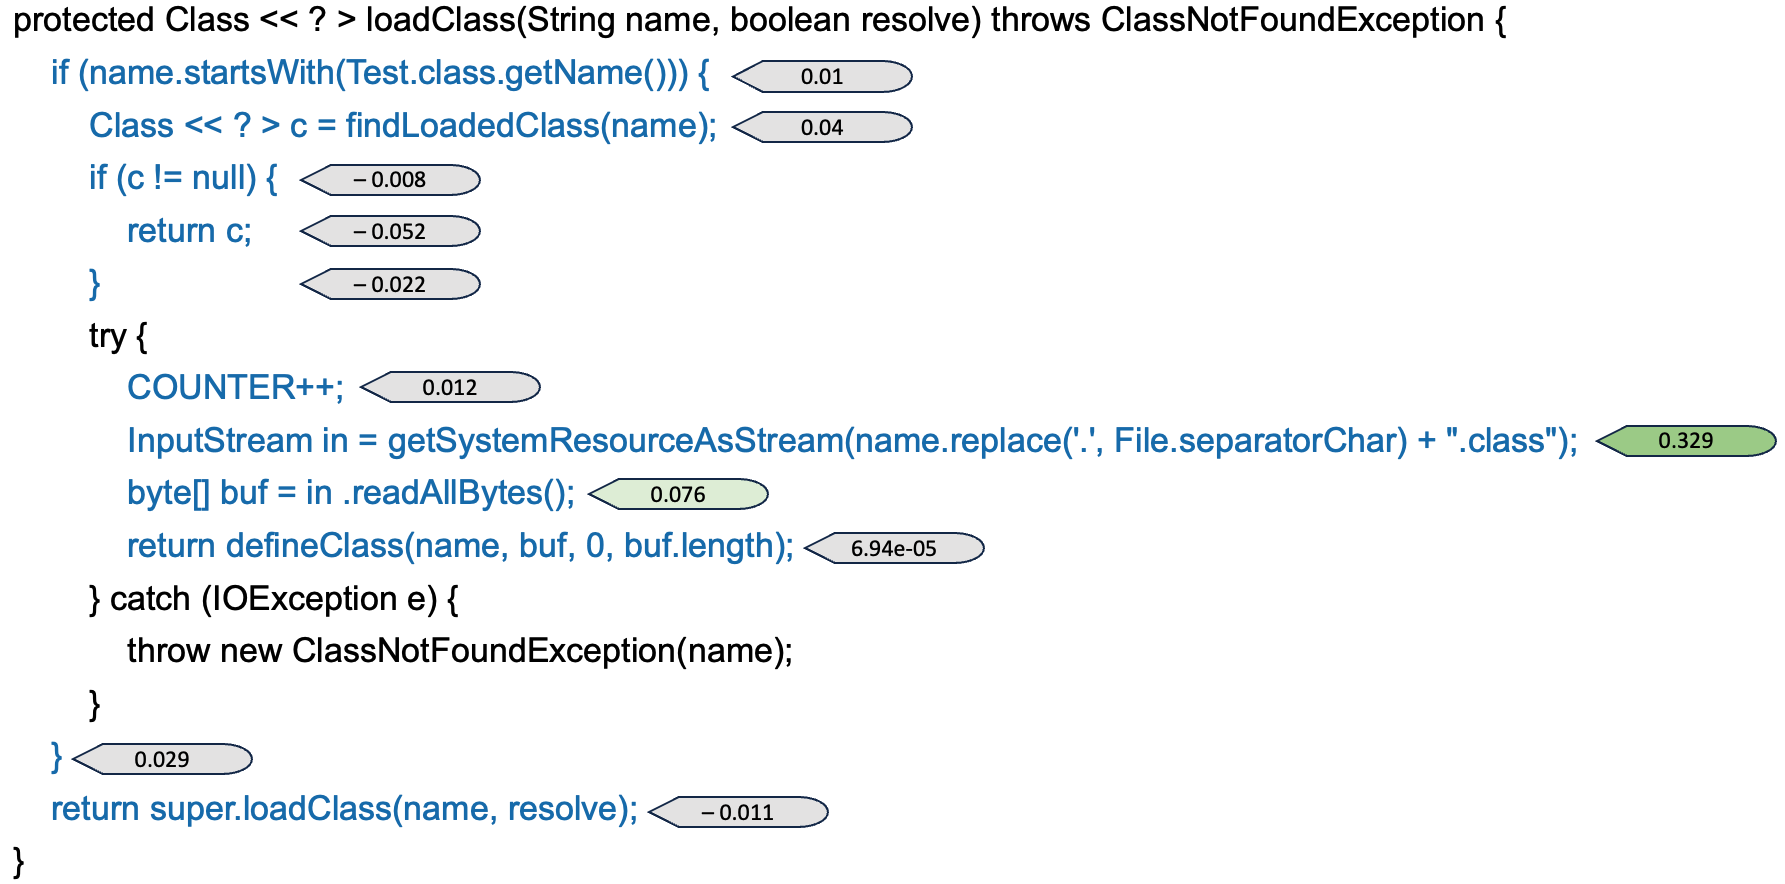
\includegraphics[width=3.4in]{rq1-case-study.png}
        \vspace{-20pt}
 	\caption{{\xblock} Case Study}
 	\label{fig:rq1-case}	
\end{figure}

\noindent {\bf Attribution Scores.} To illustrate how {\xblock} makes
the prediction, in Figure~\ref{fig:rq1-case}, we shows a code snippet
that catches an \code{IOException} thrown by the \code{readAllBytes}
API call on an \code{InputStream} object. CodeBERT produces as a
by-product an {\em attribution score} for each code sub-token in the
input. The higher the score of a token the higher attention that the
model pays to that token, contributing to the prediction result. In
Figure~\ref{fig:rq1-case}, for each statement, we show the statement
attribution score, which is calculated by averaging the attribution
scores of all the sub-tokens in the statement.
%The number after each statement is the statement attribution score,
%which is calculated by averaging the attribution scores of all the
%sub-tokens in the statement.
%
A positive attribution score means that the statement contributes
positively to the model's predicted class, while a negative score
means the statement contributes negatively to the predicted class.  As
seen, the two statements that receive the highest scores are the
statement that defines the \code{InputStream} variable and the
statement that invokes the \code{readAllBytes} method call on the
\code{InputStream} object. This example illustrates that the model is
able to put the attention on the right (sub)tokens of those statements
including \code{InputStream}, \code{in}, \code{get}, \code{System},
\code{name}, \code{replace}, etc., leading to its correct prediction.

%to decide the need of the \code{try-catch} block.
